\chapter{Installation des Betriebssystem}
\section{Cluster-Layout}
\begin{figure}[H]
	\centering
	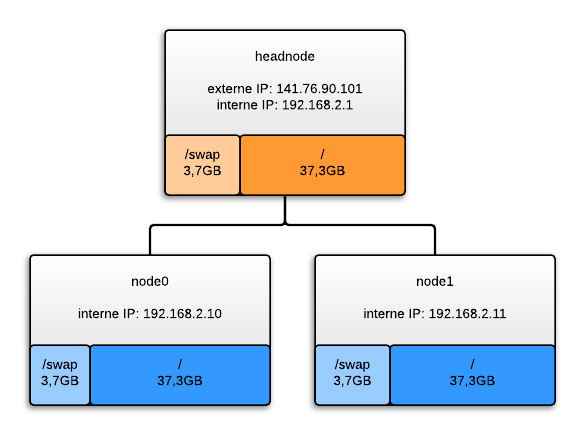
\includegraphics[width=400px]{cluster_layout.png}
	\caption{Cluster Layout}
\end{figure}
Als externe IP wurde die 141.76.90.101 zugewiesen. Die Knoten werden fortlaufen von 192.168.2.10 adressiert. Knoten N bekommt die IP 192.168.2.n+10.
So lässt sich leicht erkennen zu welchem Knoten eine IP gehört.
/home und /shared befinden sich auf dem Headnode und werden auf alle Nodes exportiert. In /shared werden Tools, Compiler und Environment Modules gespeichert.\\
\section{Betriebssysteminstallation}
Es wurden alle User per Hand hinzugefügt. In /etc/sudoers wurden Superuserrechte vergeben.\\
ssh-keys wurden mit wget runtergeladen und in authorized\_keys geschrieben. Nun können sich alle Nutzer mit ihrem ssh Private Key ohne Passwort auf dem Headnode einloggen.
\begin{lstlisting}[style=Bash]
$ wget http://lctp.zih.tu-dresden.de/key/<username>.key
$ cat <username>.key >> ~.ssh/authorized_keys
\end{lstlisting}
\section{SSH-Server}
Es wurde sich für den SSH-Server Open-ssh entschieden. Um unautorisierten Zugang zu verhindern, werden zunächst alle hosts für den login gesperrt:
\begin{lstlisting}[style=Bash]
# vim /etc/hosts.deny
§\dotfill§
sshd: ALL
\end{lstlisting}
Loginversuche aus dem Uninetz werden erlaubt:
\begin{lstlisting}[style=Bash]
# vim /etc/hosts.allow
§\dotfill§
sshd: 141.76.0.0/255.255.0.0
sshd: 141.30.0.0/255.255.0.0
sshd: 192.168.2.0/255.255.255.0
sshd: LOCAL 
\end{lstlisting}

Im SSH-Server wird dies auch konfiguriert:
\begin{lstlisting}[style=Bash]
# vim /etc/ssh/sshd_config
§\dotfill§
PermitRootLogin no
RSAAuthentication yes
PubkeyAuthentication yes

AllowUsers *@141.76.*.*
AllowUsers *@141.30.*.*
AllowUsers *@192.168.2.*.*
AllowUsers *@localhost
# SSH server auf den nodes:
UseDNS no
\end{lstlisting}
Für ein passwortloses einloggen auf den Nodes wird für jeden User ein ssh Key erstellt. Da das /home Verzeichnis mit den Nodes geteilt wird, muss der Schlüssel 
nicht weiter verteilt werden:
\begin{lstlisting}[style=Bash]
$ ssh-keygen -b 1024 -N ''
$ cat ~.ssh/id_rsa.pub >> ~./ssh/authorized_keys
\end{lstlisting}
Die Nutzererstellung wurde per Script automatisiert:
\lstinputlisting[style=Bash]{../aufgabe1/addusers.sh}
\section{Parallel Distributed Shell}
PDSH ist eine verteilte Shell mit welcher Befehle auf beliebig vielen Rechnern ausgeführt werden können. So kann mit einem Befehl auf allen Nodes
Updates installiert werden.\\
Konfigurationsunterschiede zwischen den Nodes können so vermieden werden.\\
\section{Git Server}
Zur Projektverwaltung und zum dokumentieren von /etc Änderungen wird Git genutzt.
Im Home Verzeichnis des Users git wird ein Repository erstellt in welchem alle Logs, Konfigurationen und Aufgabenlösungen gespeichert werden.\\
configs Repository anlegen:
\begin{lstlisting}[style=Bash]
# su git
# mkdir configs
# cd configs && git --bare init
\end{lstlisting}
ssh-key von allen Usern zu /home/git/.ssh/autorized\_keys hinzufügen:
\begin{lstlisting}[style=Bash]
# su user
# ssh-keygen
# ssh-copy-id -i ~/.ssh/id\_rsa.pub git@localhost
\end{lstlisting}
Nun können alle User das Repository clonen:\\
\begin{lstlisting}[style=Bash]
# git clone git@localhost:configs
\end{lstlisting}
Der etc Baum ist als Submodule in configs eingebunden. Nach dem clone muss dieses initialisiert und geupdated werden:
\begin{lstlisting}[style=Bash]
# git submodule init
# git submodule update
\end{lstlisting}
\subsection{etckeeper}
Mit etckeeper werden alle Änderungen in /etc in einem git Repository eingecheckt.\\
Konfigurieren:
\begin{lstlisting}[style=Bash]
# cd /etc && git remote add git@localhost:current_etc
\end{lstlisting}
Mit Hilfe eines Hooks wird bei einem Commit automatisch gepuscht.\\
/etc/.git/hooks/config:
\begin{lstlisting}[style=Bash]
#!/bin/sh
git push origin master
\end{lstlisting}
\subsection{/var/log/* check in}
Logs werden periodisch in das git Repository eingecheckt.\\
/var/log/* wird mit einem Script in /root/chekin\_logs.sh nach git@localhost:configs gepusht:
\begin{lstlisting}[style=Bash]
#!/bin/sh
cd /root/configs
git pull
cp /var/log/* logs/ -r
git add logs/*
git commit -am "add daily logs"
git push
\end{lstlisting}
Dieses Script wird per cronjob jeden Tag um 18:05 ausgeführt:
\begin{lstlisting}[style=Bash]
# m h  dom mon dow   command
05 18 * * * /root/checkin_logs.sh
\end{lstlisting}
\section{BurnIn}
Der BurnIn wird als Hardwarestresstest genutzt. Um Lüftungs und Kühlungsprobleme zu erkennen werden beide Cores für 24 Stunden unter Vollast betrieben.\\
Der Temperaturverlauf wird während des Tests aufgezeichnet und anschließend per Script graphisch dargestellt.\\
Der BurnIn wird mit einem Script in configs/BurnIn/stresstest.sh ausgeführt.\\
Da die genutzte CPU 2 Kerne hat, wird burnP6 zweimal gestartet.\\
Die While Schleife gibt periodisch den geparsten output von sensors mit einem Zeitstempel aus:
\begin{lstlisting}[style=Bash]
#!/bin/sh
burnP6 &
burnP6 &
`sleep 24h && killall burnP6` &

while [ "`pgrep burnP6 &>/dev/null`" ]
do
        printf "%s %s\n" "`date +%d/%m/%Y\ %H:%M:%S`" "`sensors | \
		grep C | awk -F'[:|(]' '{print $2}' | \
		grep -o '[0-9]*\.[0-9]' | cut -f1 | xargs`"
        sleep 80s
done
\end{lstlisting}
Der Test wird mit screen gestartet. Dies stellt sicher dass das Script weiterläuft wenn der ssh-user sich ausloggt:
\begin{lstlisting}[style=Bash]
# screen -dm  `./stresstest.sh > sensors.txt`
\end{lstlisting}
Die Messwerte werden mit gnuplot graphisch dargestellt:
\begin{lstlisting}[style=Bash]
#!/usr/bin/gnuplot
reset
set terminal png size 1920,1080

set xdata time
set timefmt "%d/%m/%Y %H:%M:%S"
set format x "%H:%M"
set xlabel "time"

set ylabel "Temperature in C"
set yrange [20:55]
set title "cpuburn temperature"
set key reverse Left outside
set grid
set style data linespoints

plot "sensors.txt" using 1:6 title "Core 0", \
"" using 1:7 title "Core 1"
\end{lstlisting}
\newpage
\begin{figure}[H]
	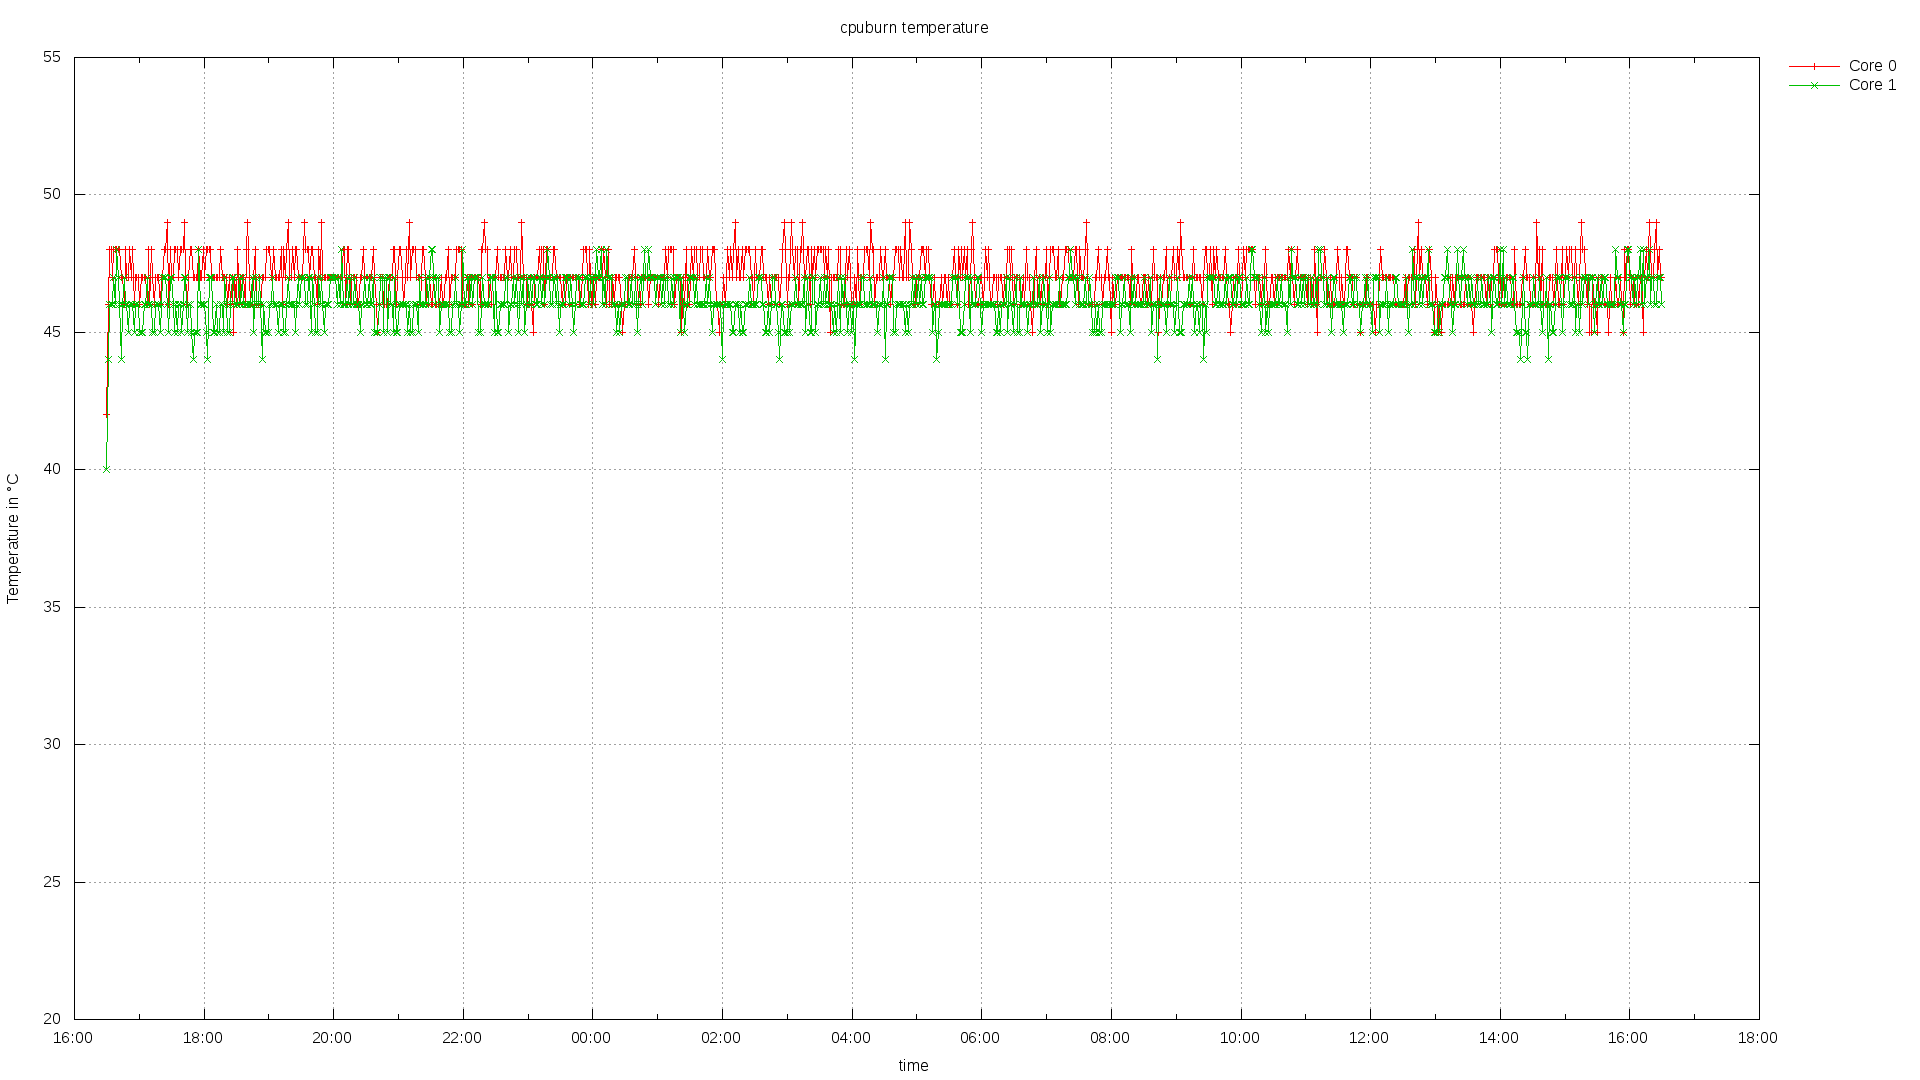
\includegraphics[scale=0.27]{../aufgabe1/BurnIn/plot.png}
	\caption{BurnIn Temperaturverlauf}
\end{figure}
